

Use an appendix to include supplementary materials that support the main content of the thesis, such as detailed calculations, additional figures, raw data, or extended explanations, ensuring the thesis remains concise and focused while providing access to relevant information for interested readers.


\section{A First Section for the Appendix}
\label{App:Appendix 1}

The Linear Dilemma matrix $M$ and the vector of inertial torques $b$, used in the simulation, are calculated as per the formulation below:

\begin{equation}
M = \left[ \begin{array}{ccc}
M_{11} & M_{12} & M_{13} \\
M_{21} & M_{22} & M_{23} \\
M_{31} & M_{32} & M_{33}
\end{array} \right]
\label{eq:dilemma_matrix}
\end{equation}

Equation~\ref{eq:dilemma_matrix} represents the Linear Dilemma matrix, which is essential for simulating the system dynamics.

\begin{figure}[h]
\centering
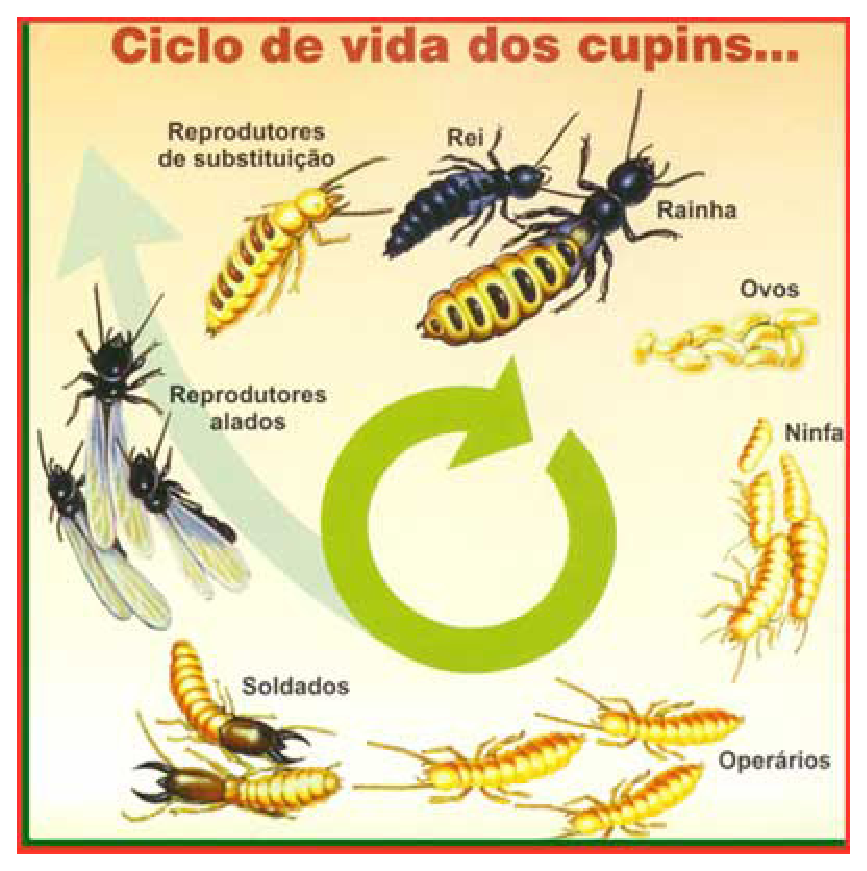
\includegraphics[height=5cm, width=5cm]{ApeA/pragas_ciclo_cupim}
\caption{An illustrative figure included in the appendix.}
\label{fig:example_figure}
\end{figure}

As shown in Figure~\ref{fig:example_figure}, the simulation involves detailed graphical representations to support the findings discussed in the main thesis.

